\documentclass{article}
\usepackage[main]{neurips_2026}
\usepackage[utf8]{inputenc}
\usepackage[T1]{fontenc}
\usepackage{hyperref,url,booktabs,amsmath,amssymb,amsthm,graphicx,microtype,xcolor}
\hypersetup{colorlinks=true,citecolor=blue,linkcolor=blue,urlcolor=blue}
\newtheorem{proposition}{Proposition}
\newtheorem{corollary}{Corollary}
\newcommand{\E}{\mathbb E}
\newcommand{\Var}{\operatorname{Var}}
\newcommand{\one}{\mathbf 1}
\newcommand{\R}{\mathbb R}
\newcommand{\RegEightRMSE}{0.197}
\newcommand{\RegDenseRMSE}{0.777}
\newcommand{\RegDenseQuad}{6.872}
\newcommand{\StanCountBias}{-0.898}
\newcommand{\StanCountRMSE}{0.033}
\newcommand{\EgoCorrCoverage}{0.480}
\newcommand{\EgoKnownCoverage}{0.950}
\newcommand{\RegDenseFit}{0.000}
\newcommand{\RegDenseBias}{-1.000}
\newcommand{\WSClusterThresholdBias}{-0.986}
\newcommand{\MainAssignments}{12,000}
\newcommand{\AllAssignments}{24,000}
\newcommand{\DenseVisibilityBound}{9.67e-10}
\newcommand{\MainSeconds}{241.1}

\title{When Regression GATE Estimates Fail:\\Endpoint Support, Contrast Leverage, and Symmetry}
\author{Anonymous Authors}
\begin{document}
\maketitle
\begin{abstract}
Regression estimators of the global average treatment effect (GATE) extrapolate from a mixed treatment assignment to two global endpoints. How reliable is that extrapolation? We conduct a fixed-graph error audit rather than propose a universally superior estimator. A finite-sample decomposition separates conditional endpoint bias from covariance-weighted contrast leverage. A support counterexample shows why observed fit alone cannot certify accuracy; a complement-symmetry result explains why balanced experiments can conceal quadratic misspecification. Across \AllAssignments{} simulated experiments on controlled synthetic networks and two public topologies, larger degree increases variance at fixed size, unnecessary but correctly specified features can sharply increase error, and count-versus-fraction misspecification is consequential on heterogeneous graphs. A threshold mechanism can have essentially zero observed signal residual yet a missing global spillover effect. Correlated errors with unit marginal variance invalidate iid regression intervals; known covariance repairs this only when contrast bias is absent. Clustering improves some settings but is not uniformly beneficial. We report Monte Carlo uncertainty, estimator availability, and rare-exposure limitations, and release the full simulation and reporting code. Conclusions concern the stated response classes and fixed graphs, not arbitrary interference or real-platform effects.
\end{abstract}

\section{Introduction}
A platform often wants the effect of treating everyone, not the direct effect of treating one user while most neighbors remain untreated. With network interference, these are different targets. A regression plug-in estimator fits outcomes against own treatment and assignment-derived neighborhood features, evaluates the fitted response under all-treatment and all-control assignments, and subtracts the predictions. This makes the target explicit, but transports a fitted relationship outside much of its observed feature support.

Prior work establishes regression adjustments for this problem and demonstrates the usefulness of appropriate interference features \citep{chin,han}. Exposure-weighted alternatives trade modeling assumptions for exposure probabilities and dependence conditions \citep{aronow,ugander}. These results do not imply that a low training error, a large sample, or a correctly included feature is individually sufficient for accurate GATE estimation. In particular, dense networks can concentrate neighbor treatment fractions around the allocation probability, making an endpoint contrast weakly informed even when outcomes are easy to predict locally.

This study asks a narrower, experimentally answerable question: \emph{for fixed-feature linear regressions, which failure mechanisms determine endpoint error, and which apparently favorable diagnostics can be misleading?} We separate three issues: endpoint transport bias, contrast-specific noise amplification, and uncertainty calibration. Availability---whether an estimator can be computed at all---is reported separately. Our primary evidence is a controlled degree/size sweep, prespecified functional misspecifications, graph-design comparisons, and two public topologies with synthetic outcomes. The additive response and Gaussian error assumptions are deliberate controls, not descriptions of an actual platform.

The contributions are an integrated error audit: (i) a standard finite-sample linear-estimator decomposition used to distinguish modeling error from noise, with a lack-of-support counterexample; (ii) a complement-symmetry argument showing why quadratic misspecification can be unbiased in balanced designs while remaining high-risk; and (iii) fully reproducible, uncertainty-qualified comparisons across feature sets, designs, degrees, graph classes, and error dependence. The algebra is elementary; we do not claim that OLS variance formulas or support concerns are new. Nor do we claim exhaustive literature novelty: an explicit independence constraint restricts literature access to permitted originals (Appendix~\ref{app:access}). The value is the jointly controlled evidence and its failure boundaries, not a new universally best estimator.

\section{Related work}
\paragraph{Regression adjustment.}
\citet{chin} fits treatment-arm-specific response regressions using interference features and predicts the global endpoints. Linear results require exogeneity and appropriate rank conditions, with stronger assumptions for variance formulas. Our arm-specific fixed-feature regressions belong to this family; pooled additive regression is a lower-dimensional restriction. We do not reproduce the source paper's complete simulation program or nonlinear procedure. \citet{han} generates graph/assignment covariates and selects them using ReFeX-LASSO, with a selection-aware graph-block bootstrap. The formal consistency result concerns the post variant under sparse linear representation and design assumptions; arbitrary feature generation is not unrestricted identification. We use known, fixed candidate maps to isolate their costs, not an implementation of ReFeX-LASSO or its bootstrap.

\paragraph{Exposure and experimental design.}
\citet{aronow} develops exposure-mapping-based randomized inference, requiring correctly mapped exposures and their probabilities. \citet{ugander} shows how graph-cluster randomization can improve full-neighborhood exposure probabilities under graph/design conditions. We include exact marginal-probability full-exposure Horvitz--Thompson (HT) and fractional H\'ajek benchmarks, while distinguishing target misspecification, empty denominators, and rare tails. Our bounded-size greedy BFS partition is not their 3-net algorithm. Our contribution does not assert that this partition optimizes a design or that clustering uniformly reduces GATE risk.

\section{Setting and error accounting}\label{sec:method}
Let $G$ be a fixed simple, undirected, unweighted graph with $n$ nodes, no isolates, adjacency $A$, degrees $d_i$, and row-normalized adjacency $P$. For assignment $z\in\{0,1\}^n$, the neighbor fraction is $s=Pz$. Potential outcomes are
\begin{equation}\label{eq:potential}
Y_i(z)=m_i(z)+\epsilon_i,\qquad \E[\epsilon\mid Z]=0,\quad \Var(\epsilon\mid Z)=\Sigma.
\end{equation}
The same error schedule is used at every potential assignment within an experiment. Thus the finite-population target is
\begin{equation}\label{eq:gate}
T=\frac1n\sum_i\{Y_i(\one)-Y_i(0)\}=\frac1n\one^\top\{m(\one)-m(0)\}.
\end{equation}
Assignments and error schedules are redrawn independently across Monte Carlo experiments. Reported coverage integrates both sources: it is not a randomization-only confidence guarantee for one fixed realized schedule.

Let $\Phi(z)\in\R^{n\times k}$ be fixed, outcome-independent features, with global contrast $c=n^{-1}\{\Phi(\one)-\Phi(0)\}^{\top}\one$. For a full-column-rank realized matrix $X=\Phi(Z)$,
\begin{equation}\label{eq:ols}
\widehat T=c^\top(X^\top X)^{-1}X^\top Y=w^\top Y,\qquad w=X(X^\top X)^{-1}c.
\end{equation}
Full column rank is our implementation rule, not a necessary condition for every identifiable contrast. We reject all singular fits rather than silently choosing a pseudoinverse prediction.

\begin{proposition}[Conditional error accounting]\label{prop:error}
Under \eqref{eq:potential}, for any working coefficient $\beta$, let $r(z)=m(z)-\Phi(z)\beta$ and $\Delta r=n^{-1}\one^\top\{r(\one)-r(0)\}$. On a full-rank assignment,
\begin{align}
\widehat T-T&=w^\top r(Z)-\Delta r+w^\top\epsilon,\label{eq:residual}\\
b(Z)&=\E[\widehat T-T\mid Z]=w^\top m(Z)-T,\nonumber\\
\E[(\widehat T-T)^2\mid Z]&=b(Z)^2+w^\top\Sigma w.\label{eq:mse}
\end{align}
Under iid errors of variance $\sigma^2$, the variance is $\sigma^2L(Z)$, where $L(Z)=\|w\|^2=c^\top(X^\top X)^{-1}c$.
\end{proposition}
The proof substitutes $w^\top X=c^\top$ and takes first and second moments; no Gaussianity is needed. The full proof and ridge qualification appear in Appendix~\ref{app:proof}. Averaging \eqref{eq:mse} over accepted assignments requires positive acceptance probability and gives $\E[b^2+v\mid\mathrm{accepted}]$, not $\E[b\mid\mathrm{accepted}]^2+\E[v\mid\mathrm{accepted}]$. Variation of conditional bias is itself risk.

A useful but non-identifying sensitivity bound is
\begin{equation}\label{eq:bound}
|b(Z)|\leq \sqrt{L(Z)}\|r(Z)\|+|\Delta r|.
\end{equation}
The endpoint residual $\Delta r$ is unobserved. Even zero in-assignment signal residual cannot validate it. The decomposition is an oracle audit in simulations, where $m$ and $T$ are known; it is not an estimator of unknown causal bias from real experimental data.

\subsection{A support obstruction}
\begin{proposition}[Indistinguishable endpoints]\label{prop:support}
On $K_n$, even $n\geq4$, randomize exactly $n/2$ treated nodes. The two response worlds $m_i^0(z)=z_i$ and $m_i^1(z)=z_i+\delta\one\{s_i(z)\geq.8\}$, $\delta>0$, have identical observed distributions but GATEs $1$ and $1+\delta$. Any everywhere-defined estimator with finite second moment has maximum MSE over these worlds at least $\delta^2/4$.
\end{proposition}
Indeed, observed $s_i\leq n/[2(n-1)]\leq2/3$, so the extra term is never seen; at global treatment it equals $\delta$. The squared-error lower bound follows by completing the square around the midpoint of the two targets. This result applies to the stated design and response class, not all Bernoulli experiments. OLS itself is singular for $(1,z,s)$ in this example.

Bernoulli assignment has positive but possibly negligible support. For a $d$-regular graph under independent probability $1/2$ assignment, a union bound gives
\begin{equation}\label{eq:visibility}
\Pr(\exists i:s_i\geq .8)\leq \min\{1,n\Pr[\mathrm{Bin}(d,.5)\geq\lceil .8d\rceil]\}.
\end{equation}
At $n=1000,d=128$, the computed upper bound is $9.67\times10^{-10}$. This is unconditional; it cannot be transferred unchanged to rank-filtered assignments. It explains why merely supplying the correct threshold feature can still leave no estimable coefficient.

\subsection{Balanced symmetry can hide curvature}\label{sec:symmetry}
\begin{proposition}[Quadratic cancellation]\label{prop:symmetry}
Let $\Phi(z)=(\one,x,z,s(z))$, with fixed $x$, and $m(z)=a\one+bx+z+s(z)^2$. Under a complement-symmetric assignment law, additive OLS GATE is unbiased conditional on full rank, provided this event has positive probability.
\end{proposition}
Complementation sends $(z,s)$ to $(1-z,1-s)$ and the regression weight $w$ to $-w$. The conditional bias is $w^\top s^2-1$ and changes sign under complementation. Full rank is invariant, so pairing assignments proves the claim (Appendix~\ref{app:symmetry}). Both Bernoulli(.5) and independent cluster(.5) assignment are symmetric. This does not imply low variance, unbiasedness for general nonlinear effects, or validity at allocation probabilities .2/.8. A balanced quadratic benchmark is therefore an insufficient stress test of endpoint transport.

\section{Experimental protocol}\label{sec:experiments}
\paragraph{Graphs and assignments.}
The main suite uses $n=1000$ random regular graphs of degree $8,32,128$, a four-block SBM with expected degree approximately $32$ (80\% within-block contribution), BA graphs with 16 new edges per node, and WS graphs of degree 32 with rewiring probability .1. Each has three fixed graph seeds, 11/23/37. Public topologies are SNAP's combined ego-Facebook network ($4039$ nodes, $88234$ edges) and Stanford3 ($11586$, $568309$), with dataset snapshots hash-verified against the supplied versions \citep{snap,nr,traud}. They are distinct collections, not two samples of one graph population. We use topology only and synthesize all outcomes and covariates. Graph statistics are in Table~\ref{tab:graphs} (Appendix~\ref{app:protocol}).

We compare independent node Bernoulli(.5) assignments with independently randomized graph blocks at probability .5. Blocks are deterministically constructed once by degree-ordered BFS, capped at 32 nodes. Between-block edges are retained. For each of 20 main graph instances and each design, we run 300 assignments, totaling \MainAssignments{} experiments. Prespecified sensitivities use 200 assignments per cell: regular graphs with $n=500/2000$ at the same degrees, and allocation probabilities .2/.8 on regular32 and WS32, again three graph seeds. Main plus sensitivities total \AllAssignments{} assignments. RNG streams are reproducible but distinct across designs/suites; different designs are not analyzed as paired draws.

\paragraph{Response mechanisms.}
A fixed covariate $x$ combines centered $\log(1+d_i)$ with independent Gaussian node variation, standardized to mean zero and variance one. Every mechanism has $m_i(z)=.5x_i+z_i+h_i(z)$, with
\begin{equation}\label{eq:mechanisms}
h_i\in\{0,\ s_i,\ s_i^2,\ \one\{s_i\geq.8\},\ t_i,\ (d_i/\bar d)s_i\},\qquad
t_i=\frac{(P^2z)_i-(P^2)_{ii}z_i}{1-(P^2)_{ii}}.
\end{equation}
Here $t$ is a normalized two-step exposure excluding returns to the same node, not a uniform average over distinct distance-two neighbors. All retained graphs have nonzero denominators. GATE is analytically 1 for no interference and 2 otherwise. A seventh mechanism repeats linear spillover with correlated noise. Default noise is iid $N(0,1)$; correlated noise is
\begin{equation}\label{eq:noise}
\epsilon=D(I+2P)u,\quad u\sim N(0,I),\quad D_{ii}=(1+4/d_i)^{-1/2}.
\end{equation}
Every marginal error variance is still one. Sharing assignments and $u$ across mechanisms and estimators supports within-design paired comparisons; it does not create independent additional replications.

\paragraph{Estimators and ablations.}
DIM is the own-treatment mean difference. Add regresses on $(1,x,z,s)$. Lin fits separate-arm linear regressions on $(1,x,s)$, equivalently pooled $(1,x,z,zx,s,zs)$. Quad adds $s^2$ in each arm; TwoHop adds $t$ to Lin; Count replaces $s$ by $(d/\bar d)s$ in Lin. This replacement avoids duplicate columns on regular graphs. Oracle uses only $(1,x,z,h)$ for the true mechanism (or $(1,x,z)$ without interference); it is an infeasible information benchmark, not a deployable method. RidgeQuad uses Quad with penalty one on raw-coordinate coefficients except the intercept. The penalty is fixed before the main study; no endpoint truth is used for tuning. These feature removals/substitutions isolate specification and variance costs without claiming data-adaptive model selection.

H\'ajek80 contrasts own-treated nodes with at least 80\% treated neighbors against own-control nodes with at most 20\% treated neighbors, weighted by exact marginal exposure probabilities. It returns unavailable if either weighted denominator is zero. HTfull uses full closed-neighborhood exposure and exact marginal propensities; it is unbiased for the one-hop mechanisms under positive propensities, but not generally for the two-hop mechanism. Under cluster assignment probabilities account for the clusters intersecting the closed neighborhood; fractional probabilities use a weighted Bernoulli convolution. These are target-qualified baselines, not automatically valid alternatives under arbitrary interference.

\paragraph{Metrics, uncertainty, and missingness.}
Primary risk is GATE RMSE, supplemented by bias, empirical SD, conditional $b^2$ and $v$, signal residual RMSE, availability, and interval coverage. OLS/ridge nominal intervals use the normal .975 quantile and residual variance times $\|w\|^2$; known-covariance intervals replace that variance by $w^\top\Sigma w$. Ridge intervals are a diagnostic, not justified unbiased regression inference. Residual-variance intervals are not implemented for DIM or exposure estimators. Raw outputs also include a generic known-noise interval diagnostic for their linear-in-outcome weights; it does not include randomization variability or confer valid GATE inference, and HT zero-weight intervals can be degenerate. Known-covariance coverage is only expected nominal with zero conditional contrast bias and positive variance.

We retain every attempt and report failures separately. Performance conditional on valid outputs must be read with availability; empty cells are not zero risk. For each fixed graph seed, MCSEs use independent assignments. Displayed synthetic aggregates describe a fixed three-graph mixture; mean-error and MSE MCSEs are stratified by graph seed, and RMSE uses the delta method. Tables show one MCSE; plotted error bars are approximate 95\% Monte Carlo intervals. Coverage/availability use Wilson intervals; per-seed metrics and denominators are released. Successful-fit mixtures can reweight graphs when availability differs. These intervals do not quantify uncertainty over a graph population. No null-hypothesis or familywise superiority claims are made; all mechanisms and negative findings are retained. Rare-exposure heavy tails can defeat empirical MCSE diagnostics entirely.

\section{Results}\label{sec:results}
\subsection{Contrast information, not fit alone, controls precision}
Figure~\ref{fig:degree} holds graph size fixed while increasing regular degree. With correct additive linear features, Bernoulli RMSE increases from \RegEightRMSE{} at degree 8 to \RegDenseRMSE{} at degree 128. Noise-integrated risk $\E[v]$ closely tracks empirical MSE; all 16 main Add/linear graph--design decomposition gaps lie within 1.96 MCSE of zero. This is a simulation check of the implementation, not evidence replacing Proposition~\ref{prop:error}.

\begin{figure}[t]
\centering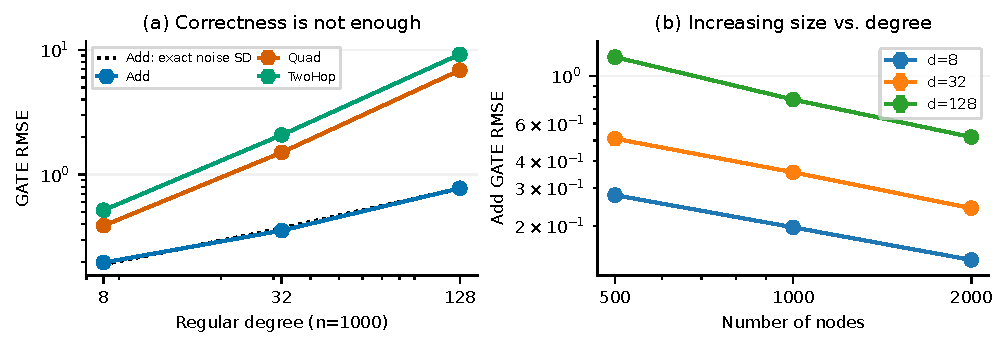
\includegraphics[width=\linewidth]{figures/degree.pdf}
\caption{Correct linear outcome mechanism, Bernoulli(.5) assignment. Left: increasing degree at fixed $n=1000$ inflates contrast variance; adding unnecessary quadratic or two-hop features further increases risk even though the models contain the truth. The dotted line is $\sqrt{\E[\|w\|^2]}$ for Add, not a fitted trend. Right: larger $n$ reduces Add risk at each fixed degree. Points summarize three fixed graph seeds; bars are approximate 95\% assignment/noise Monte Carlo intervals, not graph-population intervals.}\label{fig:degree}
\end{figure}

A well-specified but unnecessarily flexible regression is not automatically better: Quad's degree-128 linear-mechanism RMSE is \RegDenseQuad{}, despite its correctly included linear surface. Regular32's paired Quad-minus-Add MSE difference is $2.139$ (MCSE $.102$, 900 common-valid assignments). For no interference, Bernoulli DIM RMSE is about $.07$ on the synthetic graphs, while introducing irrelevant neighbor features raises variance (full summaries released). Sample size helps at fixed degree, but the public-graph results cannot be inferred from degree alone: degree heterogeneity, graph structure, covariates, and size all change the realized contrast geometry.

\begin{table}[t]
\centering\small
\caption{Bernoulli(.5) GATE RMSE (one MCSE in parentheses). Column labels specify estimator and true mechanism. Synthetic entries summarize three fixed graph seeds with 300 experiments each; each public entry has 300. All displayed fits are available. These are different response settings, not a single ranking task.}\label{tab:rmse}
\begin{tabular}{lrrrrr}\toprule
Graph & Add: linear & Quad: linear & Add: 2-hop & TwoHop: 2-hop & Count: count \\ \midrule
Regular 8 & $0.197\,(0.005)$ & $0.389\,(0.009)$ & $1.036\,(0.007)$ & $0.518\,(0.012)$ & $0.197\,(0.005)$ \\
Regular 32 & $0.356\,(0.008)$ & $1.505\,(0.034)$ & $1.070\,(0.012)$ & $2.079\,(0.049)$ & $0.358\,(0.008)$ \\
Regular 128 & $0.777\,(0.019)$ & $6.872\,(0.165)$ & $1.233\,(0.023)$ & $9.216\,(0.214)$ & $0.777\,(0.019)$ \\
SBM & $0.355\,(0.008)$ & $1.499\,(0.034)$ & $1.025\,(0.012)$ & $1.588\,(0.040)$ & $0.328\,(0.008)$ \\
BA & $0.312\,(0.008)$ & $1.130\,(0.028)$ & $1.062\,(0.010)$ & $1.844\,(0.040)$ & $0.142\,(0.004)$ \\
WS & $0.362\,(0.009)$ & $1.693\,(0.044)$ & $0.613\,(0.011)$ & $0.598\,(0.014)$ & $0.363\,(0.009)$ \\
ego-Facebook & $0.108\,(0.004)$ & $0.200\,(0.008)$ & $0.790\,(0.006)$ & $0.245\,(0.010)$ & $0.048\,(0.002)$ \\
Stanford3 & $0.063\,(0.003)$ & $0.106\,(0.004)$ & $0.968\,(0.004)$ & $0.224\,(0.008)$ & $0.033\,(0.001)$ \\
\bottomrule\end{tabular}
\end{table}

Table~\ref{tab:rmse} also separates two-hop misspecification from information scarcity. On Stanford3, adding $t$ substantially improves the two-hop target. On high-degree regular graphs, even the correctly specified TwoHop estimator is extremely noisy. The Oracle two-hop estimator is also high-variance there (released summaries), so this is not merely an avoidable cost of own-arm interaction terms. A heuristic population-moment proxy for Add leverage is $4(1+d)/n$, but it ignores cross-row dependence, centering, spectrum, and singularity; we use measured $L$ rather than assert this as a universal graph rate.

\subsection{Hidden endpoint effects and allocation sensitivity}
For the degree-128 threshold mechanism, Add's mean signal residual RMSE is \RegDenseFit{}, yet its noise-integrated conditional bias is \RegDenseBias{}. The observed signal is effectively indistinguishable from no spillover; the missing global threshold effect remains one. Supplying the true threshold basis does not solve absent support: Oracle succeeds on 0/900 Bernoulli assignments and only 51/900 cluster assignments. The latter conditional RMSE must not be compared as if all 900 experiments produced estimates.

\begin{figure}[t]
\centering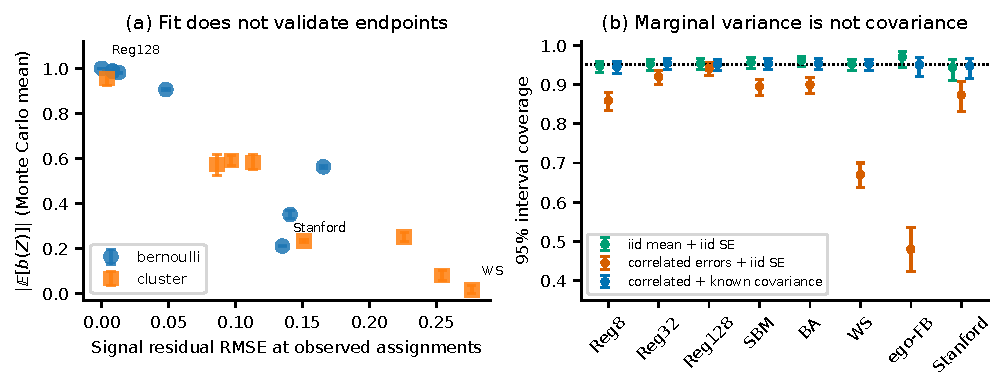
\includegraphics[width=\linewidth]{figures/failure.pdf}
\caption{Two different failure modes. (a) Add under threshold interference: absolute mean conditional endpoint contrast bias versus mean in-assignment signal residual RMSE, for eight graph classes and two designs. Selected labels identify examples; vertical bars use MCSE of the conditional bias, not outcome residuals. (b) Add under correctly specified linear means, Bernoulli assignment: iid residual intervals versus known-covariance intervals. Correlated errors have unit marginal variance throughout. Coverage bars are Wilson 95\% intervals across assignments/noise; the dotted line is .95.}\label{fig:failure}
\end{figure}

\begin{table}[t]
\centering\small
\caption{Threshold-mechanism diagnostics. B: Bernoulli; C: BFS-cluster assignment. Add bias is mean estimation error (MCSE); signal fit is residual RMSE against the noiseless observed mean. Valid/attempted counts refer to Oracle and H\'ajek80 (H80), not Add. Wilson intervals and per-seed denominators are in the released summaries.}\label{tab:support}
\begin{tabular}{llrrrr}\toprule
Graph & Design & Add bias & Signal fit & Oracle valid & H80 valid \\ \midrule
Regular 32 & B & $-0.994\,(0.012)$ & $0.008$ & 210/900 & 11/900 \\
Regular 32 & C & $-0.571\,(0.015)$ & $0.097$ & 897/900 & 894/900 \\
Regular 128 & B & $-0.956\,(0.026)$ & $0.000$ & 0/900 & 0/900 \\
Regular 128 & C & $-0.948\,(0.030)$ & $0.004$ & 51/900 & 0/900 \\
WS & B & $-0.988\,(0.012)$ & $0.008$ & 181/900 & 11/900 \\
WS & C & $0.018\,(0.010)$ & $0.277$ & 900/900 & 900/900 \\
ego-Facebook & B & $-0.359\,(0.011)$ & $0.141$ & 300/300 & 300/300 \\
ego-Facebook & C & $-0.072\,(0.011)$ & $0.254$ & 300/300 & 300/300 \\
Stanford3 & B & $-0.217\,(0.004)$ & $0.135$ & 300/300 & 300/300 \\
Stanford3 & C & $-0.239\,(0.004)$ & $0.151$ & 300/300 & 300/300 \\
\bottomrule\end{tabular}
\end{table}

Quadratic spillover produces a different lesson. At probability .5, Add often has nearly zero \emph{average} bias despite being misspecified, consistent with Proposition~\ref{prop:symmetry}. On regular32, bias is $-.005$ (MCSE $.012$). At probabilities .2/.8 it becomes $-.558$ (MCSE $.019$) and $.592$ (MCSE $.020$), respectively. Figure~\ref{fig:allocation} shows why evaluation only at balanced allocation can miss this vulnerability. Quad removes the functional misspecification but can pay a large variance cost; fixed ridge shrinks that cost while introducing its own endpoint bias. We do not select whichever estimator wins each scenario using known truth.

\begin{figure}[t]
\centering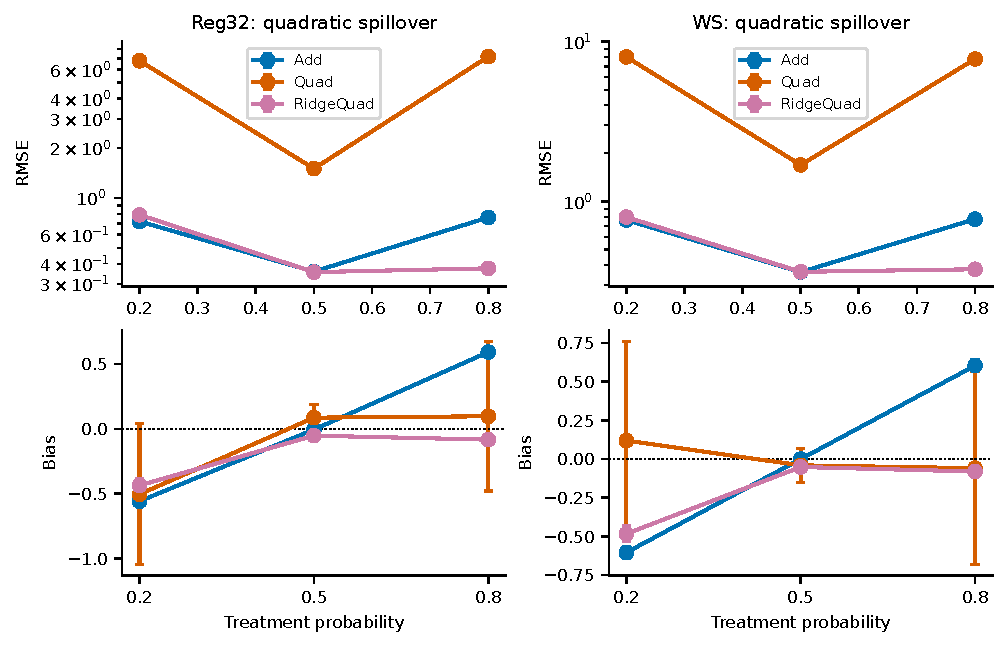
\includegraphics[width=.88\linewidth]{figures/allocation.pdf}
\caption{Prespecified allocation sensitivity under quadratic spillover, regular32 and WS32, Bernoulli assignment. Top: RMSE (log scale); bottom: bias. Add, Quad and fixed-penalty RidgeQuad exhibit different bias--variance tradeoffs. The .5 cells reuse the main suite; .2/.8 use 200 assignments per fixed graph seed, three seeds. Error bars are approximate 95\% Monte Carlo intervals.}\label{fig:allocation}
\end{figure}

Degree-dependent spillover adds another model boundary. On Stanford3, using neighbor fraction for a degree-scaled-count mechanism yields Add bias \StanCountBias{}, whereas the matched Count estimator has RMSE \StanCountRMSE{} (Table~\ref{tab:rmse}). The reverse substitution is not generally benign either. These results do not license Count as a uniformly better feature: it matches a different hypothesized response surface. On regular graphs count and fraction are scalar multiples and cannot be independently identified in a regression that includes both. Figure~\ref{fig:heatmap} gives additional feature-map comparisons, marking incomplete availability.

\subsection{Clustering and uncertainty address different problems}
Clustering improves exposure spread and some RMSEs, especially on WS, but does not uniformly dominate. BA/quadratic Add RMSE increases from $.314$ to $.378$ under our fixed cluster design, and the direction persists across all three graph seeds. Stanford3/threshold Add bias is not improved by this partition (Table~\ref{tab:support}). Clustering also changes the variability of conditional bias, so average unbiasedness need not imply calibrated intervals. We make no claims about alternative optimized partitions or maximum block sizes not studied.

With correlated errors, iid standard errors can be severely anticonservative despite the correct linear mean and unit marginal error variances. On ego-Facebook, Add coverage falls to \EgoCorrCoverage{} (Wilson 95\% interval approximately $.424$--$.536$), while using known covariance gives \EgoKnownCoverage{} (approximately $.919$--$.969$). Figure~\ref{fig:failure} distinguishes this covariance failure from endpoint misspecification. Known-covariance intervals remain non-nominal under biased response models; the benchmark is an oracle diagnostic, not an operational covariance estimator.

\paragraph{Rare exposure is not empirical unbiasedness testing.}
For regular32/Bernoulli/linear, HTfull returns zero in all 900 experiments: empirical bias is $-2$, and empirical bias MCSE is zero. Nevertheless the exact one-hop HT estimator is unbiased; the finite sample missed its enormous compensating rare tails. This is not evidence refuting the HT theorem, nor a usable precision guarantee. On Stanford3/Bernoulli, some full-exposure probabilities underflow floating point; all HTfull attempts are explicitly unavailable rather than clipped. Fractional H\'ajek has many empty exposure arms, while its nonempty estimates generally target an exposure-conditioned contrast rather than GATE for fractional nonlinear/multihop responses. Full status counts, zero-estimate fractions, and exposure diagnostics are released; unreliable rare-event RMSEs are not promoted as true-risk rankings.

\section{Discussion, limitations, and conclusion}\label{sec:limitations}
Regression GATE precision requires more than a rich predictor: the endpoint contrast must be informed by the assignment, the mean response must transport adequately, and covariance must be handled correctly. The audit suggests reporting contrast leverage, exposure range and rank availability alongside predictive diagnostics, explicitly varying plausible functional forms, and assessing allocation imbalance rather than relying only on balanced quadratic examples. These are diagnostics and sensitivity analyses, not data-only identification of the unobserved endpoint residual.

Scope is intentionally limited. The graph is known, static, unweighted, and undirected; outcome mechanisms are controlled functions with unit direct/spillover strengths. We do not study endogenous network formation, time dynamics, treatment-induced edges, real outcome heterogeneity, unknown networks, or graph-population inference. Covariance is known only for an oracle benchmark. Three synthetic graph realizations and two nonrepresentative public social topologies do not establish universal rates. Our arbitrary BFS partition and penalty are not tuned or optimal. Rank rejection can discard estimable singular contrasts; normal intervals and delta-method risk MCSEs are approximate, particularly fragile for rare-event tails. We did not implement data-adaptive ReFeX-LASSO, its block bootstrap, GNN estimators, or optimization-based designs; no comparative claim about those methods follows. The restrictive source policy prevents an exhaustive novelty assessment.

All findings are simulated; no real behavioral effect is estimated. Better network evaluation could reduce biased platform decisions, but false confidence in a model can also justify harmful global rollouts or obscure heterogeneous effects. These diagnostics should not replace domain-specific safety/fairness evaluation. Only public anonymized topology is used, with no profile attributes, reidentification, participants, or new platform data collection. Dataset license and attribution limitations are stated in Appendix~\ref{app:access}. This unattended research draft was developed with LLM assistance for hypotheses, proofs, code, analysis, and writing; execution artifacts substantiate numerical claims, but no human expert review or conference acceptance is implied. A responsible human author would still need to assess novelty, rights, and submission suitability.

\clearpage
\begin{thebibliography}{9}
\bibitem[Aronow and Samii(2017)]{aronow} Peter M. Aronow and Cyrus Samii. Estimating average causal effects under general interference, with application to a social network experiment. \emph{Annals of Applied Statistics}, 2017. Consulted original preprint v4: \url{https://arxiv.org/pdf/1305.6156}.
\bibitem[Chin(2019)]{chin} Alex Chin. Regression adjustments for estimating the global treatment effect in experiments with interference. 2019. \url{https://arxiv.org/pdf/1808.08683}.
\bibitem[Han and Ugander(2023)]{han} Kevin Han and Johan Ugander. Model-based regression adjustment with model-free covariates for network interference. 2023. \url{https://arxiv.org/pdf/2302.04997}.
\bibitem[Ugander et al.(2013)]{ugander} Johan Ugander, Brian Karrer, Lars Backstrom, and Jon Kleinberg. Graph cluster randomization: Network exposure to multiple universes. \emph{KDD}, 2013. \url{https://arxiv.org/pdf/1305.6979}.
\bibitem[Traud et al.(2012)]{traud} Amanda L. Traud, Peter J. Mucha, and Mason A. Porter. Social structure of Facebook networks. \emph{Physica A}, 2012. Consulted preprint: \url{https://arxiv.org/pdf/1102.2166}.
\bibitem[SNAP(2013)]{snap} SNAP. Social circles: Facebook, combined ego-network dataset and attribution page. Page credits J. McAuley and J. Leskovec, \emph{Learning to Discover Social Circles in Ego Networks}, NIPS 2012. Dataset file dated 2013. \url{https://snap.stanford.edu/data/ego-Facebook.html}. Accessed 2026-11-02; original article unavailable at attempted URLs, not relied upon for research claims.
\bibitem[Network Repository(2026)]{nr} Network Repository. Stanford3 dataset and repository attribution page. Credits Ryan A. Rossi and Nesreen K. Ahmed, \emph{The Network Data Repository with Interactive Graph Analytics and Visualization}, AAAI 2015. \url{https://networkrepository.com/socfb-Stanford3.php}. Accessed 2026-11-02; original repository article unavailable at attempted URL.
\bibitem[Network Repository Policy(2026)]{nrpolicy} Network Repository. Data policy and license. \url{https://networkrepository.com/policy.php}. Accessed 2026-11-02.
\end{thebibliography}

\clearpage
\appendix
\section{Proofs and boundaries}\label{app:proof}
\paragraph{Proposition~\ref{prop:error}.}
Since $X$ has full column rank, $w^\top X=c^\top$. Write $m(z)=\Phi(z)\beta+r(z)$ for every assignment, including global endpoints. Then $T=c^\top\beta+\Delta r$, while $w^\top Y=c^\top\beta+w^\top r(Z)+w^\top\epsilon$. Subtraction gives \eqref{eq:residual}. Conditional on $Z$, $w$ is fixed, $\E[w^\top\epsilon\mid Z]=0$ and its variance is $w^\top\Sigma w$. Expanding the square proves \eqref{eq:mse}. With iid variance $\sigma^2$, $w^\top w=c^\top(X^\top X)^{-1}c$ by multiplying the definition of $w$. Cauchy--Schwarz and the triangle inequality prove \eqref{eq:bound}. Conditioning on a positive-probability feature-only rank event preserves assignment--noise independence, but changes the assignment law. For a fixed graph the assignment space is finite; on accepted full-rank matrices all displayed moments exist under finite-variance noise.

For RidgeQuad, $\lambda=1$, $D_0=\operatorname{diag}(0,1,\ldots,1)$ and $w_\lambda=X(X^\top X+\lambda D_0)^{-1}c$. The penalized Gram matrix is positive definite because $X$ has a nonzero intercept and every other coefficient is penalized. Directly, $b_\lambda=w_\lambda^\top m-T$, $v_\lambda=w_\lambda^\top\Sigma w_\lambda$ still imply MSE $b_\lambda^2+v_\lambda$. However $w_\lambda^\top X=c^\top$ generally fails, so OLS residual cancellation is not asserted for ridge. A residual-variance interval need not cover a shrinkage-biased endpoint contrast.

For Gaussian noise with positive variance, the known-covariance interval centered at $w^\top Y$ has exact 95\% conditional coverage if $b(Z)=0$, using $q_{.975}=1.959963984540054$. Full correct mean specification is sufficient, not necessary, for this contrast condition. Neither Gaussianity nor known covariance eliminates nonzero $b(Z)$. Zero-variance degenerate intervals need separate treatment; our reported regression cells have positive variance.

\paragraph{Proposition~\ref{prop:support}.}
A treated node in a balanced complete graph has neighbor fraction $(n/2-1)/(n-1)$ and a control node $(n/2)/(n-1)$. For even $n\geq4$, both are below .8. Observed means are therefore identical in the two worlds at every supported assignment, as are observed distributions if the same assignment-independent noise law is added. At $\one$, the threshold is one at every node; at $0$, it is zero. Thus targets differ by $\delta$. For any real number $a$,
\[
(a-1)^2+(a-1-\delta)^2=2(a-1-\delta/2)^2+\delta^2/2.
\]
Taking expectation under the common observed law and dividing by two proves the maximum-risk bound. The triangle inequality similarly implies at least one absolute bias of $\delta/2$. This claim concerns estimators defined on all observations; an algorithm declining to estimate has availability, not an assigned MSE.

For \eqref{eq:visibility}, each node has $d$ distinct, independently assigned neighbors, so its treated-neighbor count is binomial. A union bound over nodes suffices; exposures across nodes need not be independent. If $R$ is a positive-probability rank-acceptance event, only the generic bound $\Pr(\exists i:s_i\geq .8\mid R)\leq\min\{1,np_d/\Pr(R)\}$ follows from the unconditional tail $p_d$. The original binomial law need not survive filtering.

\subsection{Complement proof}\label{app:symmetry}
For Proposition~\ref{prop:symmetry}, let $X=(\one,x,z,s)$. There is an invertible matrix $B$ with $B^2=I$, $X(\one-z)=XB$, and $B^\top c=-c$ for $c=(0,0,1,1)^\top$. Explicitly,
\[
B=\begin{pmatrix}1&0&1&1\\0&1&0&0\\0&0&-1&0\\0&0&0&-1\end{pmatrix}.
\]
Thus the complement has the same rank, and
\[
w(\one-z)=XB(B^\top X^\top XB)^{-1}c=X(X^\top X)^{-1}(B^\top)^{-1}c=-w(z).
\]
The constraints are $w^\top\one=w^\top x=0$ and $w^\top z=w^\top s=1$. Consequently $b(z)=w^\top s^2-1$. At the complementary assignment,
\[
b(\one-z)=-w^\top\{a\one+bx+(\one-z)+(\one-s)^2\}-2=1-w^\top s^2=-b(z).
\]
The positive-probability full-rank set is complement invariant. Pairing its finite assignment probabilities, which are equal by hypothesis, yields $\E[b\mid R]=0$. Independent mean-zero noise does not change this expectation. Nonlinear threshold spillover, asymmetric allocation, and ridge penalty equivariance are not covered by this proposition. The result also does not establish correct intervals: $\Var(b(Z)\mid R)$ can be positive even when its mean is zero.

\paragraph{Correlated covariance.}
For a simple unweighted graph, $P_{ii}=0$ and $\sum_jP_{ij}^2=1/d_i$, so \eqref{eq:noise} gives unit marginal variance. For any fixed $w$,
\[
w^\top\Sigma w=\|(I+2P)^\top Dw\|^2=\|Dw+2P^\top Dw\|^2.
\]
Our code uses this sparse expression rather than forming a dense covariance matrix. The two-hop feature likewise uses two sparse matvecs and the diagonal return probability; it does not build a dense $P^2$.

\section{Full implementation and reporting details}\label{app:protocol}
\begin{table}[h]
\centering\small
\caption{Main graph statistics for seed 11 (synthetic) or the fixed public graph. Full per-seed manifests are delivered. Blocks are capped at 32 but may be smaller; edge cut is the fraction of edges crossing the partition.}\label{tab:graphs}
\begin{tabular}{lrrrrr}\toprule
Graph & $n$ & Mean $d$ & Max $d$ & Blocks & Edge cut \\ \midrule
Regular 8 & 1000 & 8.00 & 8 & 54 & 0.746 \\
Regular 32 & 1000 & 32.00 & 32 & 42 & 0.915 \\
Regular 128 & 1000 & 128.00 & 128 & 33 & 0.955 \\
SBM & 1000 & 31.95 & 49 & 46 & 0.889 \\
BA & 1000 & 31.49 & 230 & 64 & 0.902 \\
WS & 1000 & 32.00 & 38 & 39 & 0.555 \\
ego-Facebook & 4039 & 43.69 & 1045 & 441 & 0.815 \\
Stanford3 & 11586 & 98.10 & 1172 & 1653 & 0.964 \\
\bottomrule\end{tabular}
\end{table}

Graphs are symmetrized, self-loops removed, and duplicate edges collapsed. Only the largest component would be kept; the reported public counts match the downloaded connected topologies. Stanford3 is the Facebook100 largest-component topology, not the SNAP ego-network union. The Stanford MatrixMarket archive has a single-percent header accepted by the installed SciPy reader. Original hashes, byte sizes, page snapshots, and source notes are in the delivered data manifest and access logs. The synthetic covariate is built using a seed distinct from assignment streams: centered $\log(1+d_i)$, standardized when nonconstant (zero on regular graphs), plus $.5$ independent normal node variation, then standardized again. Thus regular graphs retain a nonconstant covariate without claiming real profile attributes.

The SBM has four nearly equal blocks with within probability $25.6/(n/4-1)$ and between probability $6.4/(3n/4)$. BFS roots are ordered by descending degree with stable ties; each unassigned root starts a queue, taking unassigned vertices until size 32, then moving to the next root. Leftover nodes start later blocks. This fixed partition is regenerated deterministically from the saved adjacency; no response or assignment is used in clustering. The block cap is not necessarily the realized average block size.

Design matrices use raw $s,s^2,t,(d/\bar d)s$ coordinates. Eigenvalues of $X^\top X$ smaller than $10^{-10}\max(\lambda_{\max},1)$ count as numerically zero. OLS rejects deficient rank; positive-penalty ridge remains defined. Proposition~\ref{prop:symmetry} concerns exact mathematical rank: this raw-coordinate numerical cutoff need not be complement invariant. Add had no rejected fits in the reported suites, so no filtered pairs affect its reported cancellation evidence. The software records Gram condition numbers but does not select fits by condition number after full-rank acceptance. Every method recomputes its own endpoint feature contrast, including count normalization and treatment-feature interactions. Gaussian variance is estimated from residual sum of squares divided by $n-\mathrm{rank}(X)$; with ridge this is merely a diagnostic scale, not an effective-degrees-of-freedom adjustment.

For independent node assignment, full treatment/control propensities are $p^{d_i+1}$ and $(1-p)^{d_i+1}$. Fractional treated exposure requires $Z_i=1$ and neighbor count at least $\lceil .8d_i\rceil$; fractional control requires $Z_i=0$ and count at most $\lfloor .2d_i\rfloor$. Cluster full-exposure propensities replace closed-neighborhood size by the number of distinct touching clusters. Fractional cluster propensities condition on own-cluster treatment and convolve the remaining cluster weights by their neighbor counts. The final 15-test suite includes exhaustive small-graph exposure-probability checks, endpoint truths, covariance orientation, rank handling, a balanced-graph counterexample, complementary weights/biases, attempted-record ratio uncertainty, and completeness-validation rejection tests. The initial seven tests preceded the pilot; reporting tests were added after independent review. Numerical checks are not substituted for general proofs.

Each assignment uses \texttt{SeedSequence([20261102, suite, graphIndex, designIndex, rep])}, where suite codes are 0 pilot, 1 main, 2 size, and 3 allocation. Graph configuration order is defined in \texttt{run\_experiments.py}; no hash-dependent RNG seeds are used. Main results exclude the five-replicate pilot, whose realized synthetic seed was only 11 despite a generic metadata list of all three graph seeds. Designs use separate streams, and mechanisms share noise only within an assignment. Scripts overwrite their own suite output directory; the README explicitly warns against accidental reruns over archived outputs.

For all-valid records of a fixed graph, MCSE of bias is $\mathrm{sd}(e)/\sqrt{R}$, of MSE is $\mathrm{sd}(e^2)/\sqrt{R}$, and of RMSE is MSE MCSE divided by $2\sqrt{\overline{e^2}}$. With failures, pooled performance is a ratio $\widehat\theta=\sum VH/\sum V$, where $V$ indicates validity and $H$ is the metric. Its target is the equal-attempt fixed-graph mixture conditioned on validity, which reweights graph seeds by success probability. Let $U_{jr}=V_{jr}(H_{jr}-\widehat\theta)$, zero on invalid attempts. We use the attempted-record stratified delta variance $\widehat{\mathrm{SE}}^2=\sum_j R_j\mathrm{var}_r(U_{jr})/N_{\rm valid}^2$, then apply the RMSE delta transform. This includes random accepted-count variation; it reduces to ordinary fixed-stratum mean uncertainty when all records are valid. Fewer than two successes gives unavailable MCSE; fewer than 30 successes is flagged as sparse. These local asymptotic diagnostics cannot certify unseen rare tails. This formula was corrected after self-review, with the original pre-main protocol and dated reporting amendment retained; experiment designs and outcomes were not changed. Per-seed conditional estimates and availability remain supplied. Wilson coverage intervals pool independent Bernoulli indicators as a fixed-mixture approximation; per-seed intervals are also available. Paired comparisons use all attempted keys and joint validity in the same ratio calculation, within a design only.

The direct accounting check uses $D_r=e_r^2-b_r^2-v_r$ on identical valid draws. We report its mean and MCSE. All three suites validate record uniqueness, finite values for successful estimates, expected assignment counts, and availability statuses before analysis. \texttt{summary.csv} has 2520 scenario/estimator cells and \texttt{per\_seed.csv} has 7000; raw files contain 1,680,000 method--mechanism evaluations, not that many independent experiments. No rare-event trimming, pseudo-count smoothing, rank redraw, or replacement of failures by zero is performed.

\begin{figure}[h]
\centering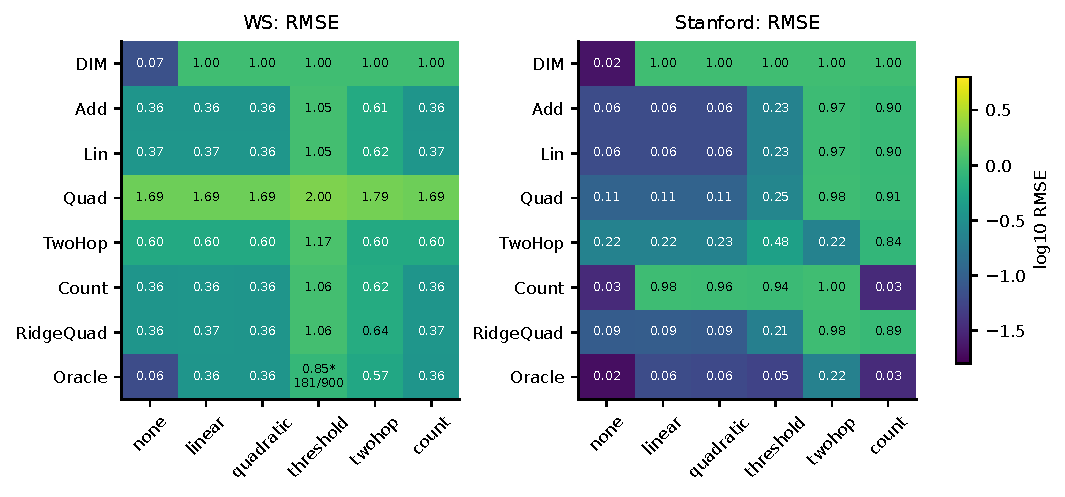
\includegraphics[width=\linewidth]{figures/heatmap.pdf}
\caption{Additional Bernoulli(.5) RMSE comparisons on WS and Stanford3. Cells use measured simulation summaries, rounded for display; color is log10 RMSE. A star and valid/attempted counts mark incomplete cells; other WS cells use 900/900 and Stanford cells 300/300. These method-conditional risks are not common-subset comparisons. Oracle is a known-true-basis benchmark, not a learned method. Monte Carlo uncertainty is supplied in the CSVs; no significance rankings follow.}\label{fig:heatmap}
\end{figure}

\paragraph{Reproducibility and compute.}
Use Python 3.11.15, NumPy 2.4.6, SciPy 1.17.1, pandas 3.0.6, NetworkX 3.4.2, Matplotlib 3.11.2, pytest 8.3.5, and pypdf 5.9.0. Main simulation uses one BLAS/OpenMP thread, no GPU, on a Linux x86-64 sandbox exposing 40 logical CPUs; the processor model is not exposed. Main wall time was \MainSeconds{} seconds; per-suite and analysis timings are delivered. These are measurements of this environment, not portability guarantees. Main peak memory was not instrumented; analysis peak RSS and environment metadata are recorded separately. The pilot and failed tooling attempts are logged. The entire research, including figures and tests, is substantially smaller than a week, but a new machine should allow additional time for package installation, graph downloads, and TeX.

The reproduction sequence is \texttt{fetch\_data.py}; \texttt{pytest}; \texttt{run\_experiments.py --suite main --reps 300}; corresponding size/allocation commands with 200; \texttt{analyze.py}; \texttt{plot\_results.py}; \texttt{prepare\_paper.py}; and \texttt{latexmk -pdf main.tex} in the paper directory. The root README supplies exact commands, runtime measurements, and every figure/table mapping. All empirical LaTeX tables/macros are generated from raw records. Analysis scripts, source code, and figure PDFs/PNGs are provided; no network access to unrelated literature is needed for reproduction.

\section{Source access, attribution, and research conduct}\label{app:access}
The task expressly prohibited an unidentified existing paper and all its mirrors, discussions, citing pages, and code. We made no attempt to identify it. To avoid indirect exposure, no topic search, citation traversal, recommendation system, literature aggregator, or repository search was used. Methodological reading was restricted to original PDFs of the four explicitly permitted papers cited above. Dataset provenance reading used the permitted Traud original and exact supplied data/policy pages. Conference access was restricted to official NeurIPS 2026 formatting instructions, template archive, and ethics guidelines. No known prohibited material was encountered. Full source requests, hashes, local reading notes, and failures are delivered; references to unrelated works inside allowed originals were not followed.

The official NeurIPS 2026 style/template/checklist were downloaded from the official CFP-linked archive. The direct StyleFiles route returned 404; this is logged rather than represented as successful. We use the unchanged \texttt{neurips\_2026.sty}, main-track anonymous mode, a nine-page main-text upper limit, and the official retained checklist questions/guidelines, with completed answers. This formatting choice is not an assertion of submission or acceptance.

Stanford3 comes from Network Repository and corresponds to the Full Stanford graph documented by Traud et al. Repository attribution is to Ryan A. Rossi and Nesreen K. Ahmed and their AAAI 2015 work, as specified by the read dataset page. The repository policy states CC BY-SA without establishing a version in the read text \citep{nrpolicy}; we retain attribution and source notices and do not assign an invented version. Stanford preprocessing only symmetrizes topology, removes self-loops/duplicate storage, and converts sparse format; any redistributed derivative remains subject to source ShareAlike terms. SNAP's read page credits J. McAuley and J. Leskovec, NIPS 2012, and does not state a license. These credits are reproduced in the dataset references rather than claiming to have read unavailable originals. Direct attempts to retrieve that article and the repository original failed; exact URLs/errors are logged. Thus complete paper-level attribution/right clearance is not certified. The portable code archive omits original/converted public graphs and provides hash-checked fetching instead. Local task copies are retained for verification. Users must resolve uncertain rights before broader redistribution.

Only topology and synthetic outcomes are analyzed. No original demographic attributes or circle labels are imported, no new identifiable dataset is created, and no participant experiment or institutional ethics clearance is claimed. The official ethics code was consulted. The LLM-assisted unattended process contributed to study design and mathematical/code drafting, not merely prose editing; this is disclosed to avoid implying human oversight. Independent subagent audits corrected an overstrong interval-necessity statement and checked rank-conditioning boundaries. Such review is not a substitute for qualified human accountability.

\clearpage
\section*{NeurIPS Paper Checklist}




\begin{enumerate}

\item {\bf Claims}
    \item[] Question: Do the main claims made in the abstract and introduction accurately reflect the paper's contributions and scope?
    \item[] Answer: \answerYes{}
    \item[] Justification: Sections 1--6 bound the claims to fixed graphs, specified response classes and model-based Monte Carlo evidence; no universal superiority or exhaustive novelty is claimed.
    \item[] Guidelines:
    \begin{itemize}
        \item The answer \answerNA{} means that the abstract and introduction do not include the claims made in the paper.
        \item The abstract and/or introduction should clearly state the claims made, including the contributions made in the paper and important assumptions and limitations. A \answerNo{} or \answerNA{} answer to this question will not be perceived well by the reviewers. 
        \item The claims made should match theoretical and experimental results, and reflect how much the results can be expected to generalize to other settings. 
        \item It is fine to include aspirational goals as motivation as long as it is clear that these goals are not attained by the paper. 
    \end{itemize}

\item {\bf Limitations}
    \item[] Question: Does the paper discuss the limitations of the work performed by the authors?
    \item[] Answer: \answerYes{}
    \item[] Justification: Section 6 and Appendices A--C discuss support, covariance, fixed-graph scope, unavailable estimators, rare tails, source restrictions and lack of human review.
    \item[] Guidelines:
    \begin{itemize}
        \item The answer \answerNA{} means that the paper has no limitation while the answer \answerNo{} means that the paper has limitations, but those are not discussed in the paper. 
        \item The authors are encouraged to create a separate ``Limitations'' section in their paper.
        \item The paper should point out any strong assumptions and how robust the results are to violations of these assumptions (e.g., independence assumptions, noiseless settings, model well-specification, asymptotic approximations only holding locally). The authors should reflect on how these assumptions might be violated in practice and what the implications would be.
        \item The authors should reflect on the scope of the claims made, e.g., if the approach was only tested on a few datasets or with a few runs. In general, empirical results often depend on implicit assumptions, which should be articulated.
        \item The authors should reflect on the factors that influence the performance of the approach. For example, a facial recognition algorithm may perform poorly when image resolution is low or images are taken in low lighting. Or a speech-to-text system might not be used reliably to provide closed captions for online lectures because it fails to handle technical jargon.
        \item The authors should discuss the computational efficiency of the proposed algorithms and how they scale with dataset size.
        \item If applicable, the authors should discuss possible limitations of their approach to address problems of privacy and fairness.
        \item While the authors might fear that complete honesty about limitations might be used by reviewers as grounds for rejection, a worse outcome might be that reviewers discover limitations that aren't acknowledged in the paper. The authors should use their best judgment and recognize that individual actions in favor of transparency play an important role in developing norms that preserve the integrity of the community. Reviewers will be specifically instructed to not penalize honesty concerning limitations.
    \end{itemize}

\item {\bf Theory assumptions and proofs}
    \item[] Question: For each theoretical result, does the paper provide the full set of assumptions and a complete (and correct) proof?
    \item[] Answer: \answerYes{}
    \item[] Justification: Section 3 states assumptions; Appendix A proves all propositions and distinguishes the leverage heuristic, ridge bias and rank-conditioned statements.
    \item[] Guidelines:
    \begin{itemize}
        \item The answer \answerNA{} means that the paper does not include theoretical results. 
        \item All the theorems, formulas, and proofs in the paper should be numbered and cross-referenced.
        \item All assumptions should be clearly stated or referenced in the statement of any theorems.
        \item The proofs can either appear in the main paper or the supplemental material, but if they appear in the supplemental material, the authors are encouraged to provide a short proof sketch to provide intuition. 
        \item Inversely, any informal proof provided in the core of the paper should be complemented by formal proofs provided in appendix or supplemental material.
        \item Theorems and Lemmas that the proof relies upon should be properly referenced. 
    \end{itemize}

    \item {\bf Experimental result reproducibility}
    \item[] Question: Does the paper fully disclose all the information needed to reproduce the main experimental results of the paper to the extent that it affects the main claims and/or conclusions of the paper (regardless of whether the code and data are provided or not)?
    \item[] Answer: \answerYes{}
    \item[] Justification: Section 4, Appendix B and the delivered README give every mechanism, feature map, assignment rule, seed, dependency and reporting command.
    \item[] Guidelines:
    \begin{itemize}
        \item The answer \answerNA{} means that the paper does not include experiments.
        \item If the paper includes experiments, a \answerNo{} answer to this question will not be perceived well by the reviewers: Making the paper reproducible is important, regardless of whether the code and data are provided or not.
        \item If the contribution is a dataset and\slash or model, the authors should describe the steps taken to make their results reproducible or verifiable. 
        \item Depending on the contribution, reproducibility can be accomplished in various ways. For example, if the contribution is a novel architecture, describing the architecture fully might suffice, or if the contribution is a specific model and empirical evaluation, it may be necessary to either make it possible for others to replicate the model with the same dataset, or provide access to the model. In general. releasing code and data is often one good way to accomplish this, but reproducibility can also be provided via detailed instructions for how to replicate the results, access to a hosted model (e.g., in the case of a large language model), releasing of a model checkpoint, or other means that are appropriate to the research performed.
        \item While NeurIPS does not require releasing code, the conference does require all submissions to provide some reasonable avenue for reproducibility, which may depend on the nature of the contribution. For example
        \begin{enumerate}
            \item If the contribution is primarily a new algorithm, the paper should make it clear how to reproduce that algorithm.
            \item If the contribution is primarily a new model architecture, the paper should describe the architecture clearly and fully.
            \item If the contribution is a new model (e.g., a large language model), then there should either be a way to access this model for reproducing the results or a way to reproduce the model (e.g., with an open-source dataset or instructions for how to construct the dataset).
            \item We recognize that reproducibility may be tricky in some cases, in which case authors are welcome to describe the particular way they provide for reproducibility. In the case of closed-source models, it may be that access to the model is limited in some way (e.g., to registered users), but it should be possible for other researchers to have some path to reproducing or verifying the results.
        \end{enumerate}
    \end{itemize}


\item {\bf Open access to data and code}
    \item[] Question: Does the paper provide open access to the data and code, with sufficient instructions to faithfully reproduce the main experimental results, as described in supplemental material?
    \item[] Answer: \answerYes{}
    \item[] Justification: The accompanying code archive contains all scripts and measured summaries. Hash-checked public-data fetching is supplied; originals are not redistributed in that archive because rights are source-specific.
    \item[] Guidelines:
    \begin{itemize}
        \item The answer \answerNA{} means that paper does not include experiments requiring code.
        \item Please see the NeurIPS code and data submission guidelines (\url{https://neurips.cc/public/guides/CodeSubmissionPolicy}) for more details.
        \item While we encourage the release of code and data, we understand that this might not be possible, so \answerNo{} is an acceptable answer. Papers cannot be rejected simply for not including code, unless this is central to the contribution (e.g., for a new open-source benchmark).
        \item The instructions should contain the exact command and environment needed to run to reproduce the results. See the NeurIPS code and data submission guidelines (\url{https://neurips.cc/public/guides/CodeSubmissionPolicy}) for more details.
        \item The authors should provide instructions on data access and preparation, including how to access the raw data, preprocessed data, intermediate data, and generated data, etc.
        \item The authors should provide scripts to reproduce all experimental results for the new proposed method and baselines. If only a subset of experiments are reproducible, they should state which ones are omitted from the script and why.
        \item At submission time, to preserve anonymity, the authors should release anonymized versions (if applicable).
        \item Providing as much information as possible in supplemental material (appended to the paper) is recommended, but including URLs to data and code is permitted.
    \end{itemize}


\item {\bf Experimental setting/details}
    \item[] Question: Does the paper specify all the training and test details (e.g., data splits, hyperparameters, how they were chosen, type of optimizer) necessary to understand the results?
    \item[] Answer: \answerYes{}
    \item[] Justification: Section 4 and Appendix B specify features, fixed penalty, no tuning, graph generation, design, repeated experiments and uncertainty calculations.
    \item[] Guidelines:
    \begin{itemize}
        \item The answer \answerNA{} means that the paper does not include experiments.
        \item The experimental setting should be presented in the core of the paper to a level of detail that is necessary to appreciate the results and make sense of them.
        \item The full details can be provided either with the code, in appendix, or as supplemental material.
    \end{itemize}

\item {\bf Experiment statistical significance}
    \item[] Question: Does the paper report error bars suitably and correctly defined or other appropriate information about the statistical significance of the experiments?
    \item[] Answer: \answerYes{}
    \item[] Justification: Tables report Monte Carlo SEs, figures show approximate 95 percent Monte Carlo or Wilson intervals, and per-seed results expose their conditional scope. Rare HT tails are explicitly not certified by empirical zero SEs.
    \item[] Guidelines:
    \begin{itemize}
        \item The answer \answerNA{} means that the paper does not include experiments.
        \item The authors should answer \answerYes{} if the results are accompanied by error bars, confidence intervals, or statistical significance tests, at least for the experiments that support the main claims of the paper.
        \item The factors of variability that the error bars are capturing should be clearly stated (for example, train/test split, initialization, random drawing of some parameter, or overall run with given experimental conditions).
        \item The method for calculating the error bars should be explained (closed form formula, call to a library function, bootstrap, etc.)
        \item The assumptions made should be given (e.g., Normally distributed errors).
        \item It should be clear whether the error bar is the standard deviation or the standard error of the mean.
        \item It is OK to report 1-sigma error bars, but one should state it. The authors should preferably report a 2-sigma error bar than state that they have a 96\% CI, if the hypothesis of Normality of errors is not verified.
        \item For asymmetric distributions, the authors should be careful not to show in tables or figures symmetric error bars that would yield results that are out of range (e.g., negative error rates).
        \item If error bars are reported in tables or plots, the authors should explain in the text how they were calculated and reference the corresponding figures or tables in the text.
    \end{itemize}

\item {\bf Experiments compute resources}
    \item[] Question: For each experiment, does the paper provide sufficient information on the computer resources (type of compute workers, memory, time of execution) needed to reproduce the experiments?
    \item[] Answer: \answerNo{}
    \item[] Justification: Appendix B records threads, platform and measured runtimes; environment and analysis RSS are supplied, but the CPU model was not exposed and peak simulation memory was not instrumented.
    \item[] Guidelines:
    \begin{itemize}
        \item The answer \answerNA{} means that the paper does not include experiments.
        \item The paper should indicate the type of compute workers CPU or GPU, internal cluster, or cloud provider, including relevant memory and storage.
        \item The paper should provide the amount of compute required for each of the individual experimental runs as well as estimate the total compute. 
        \item The paper should disclose whether the full research project required more compute than the experiments reported in the paper (e.g., preliminary or failed experiments that didn't make it into the paper). 
    \end{itemize}
    
\item {\bf Code of ethics}
    \item[] Question: Does the research conducted in the paper conform, in every respect, with the NeurIPS Code of Ethics \url{https://neurips.cc/public/EthicsGuidelines}?
    \item[] Answer: \answerNo{}
    \item[] Justification: The official ethics code was reviewed and no new human data were collected, but complete rights clearance for SNAP's unspecified license cannot be certified. Appendix C discloses this rather than asserting full compliance.
    \item[] Guidelines:
    \begin{itemize}
        \item The answer \answerNA{} means that the authors have not reviewed the NeurIPS Code of Ethics.
        \item If the authors answer \answerNo, they should explain the special circumstances that require a deviation from the Code of Ethics.
        \item The authors should make sure to preserve anonymity (e.g., if there is a special consideration due to laws or regulations in their jurisdiction).
    \end{itemize}


\item {\bf Broader impacts}
    \item[] Question: Does the paper discuss both potential positive societal impacts and negative societal impacts of the work performed?
    \item[] Answer: \answerYes{}
    \item[] Justification: Section 6 discusses better rollout decisions, false-confidence harms, fairness limitations and the need for domain-specific safety evaluation.
    \item[] Guidelines:
    \begin{itemize}
        \item The answer \answerNA{} means that there is no societal impact of the work performed.
        \item If the authors answer \answerNA{} or \answerNo, they should explain why their work has no societal impact or why the paper does not address societal impact.
        \item Examples of negative societal impacts include potential malicious or unintended uses (e.g., disinformation, generating fake profiles, surveillance), fairness considerations (e.g., deployment of technologies that could make decisions that unfairly impact specific groups), privacy considerations, and security considerations.
        \item The conference expects that many papers will be foundational research and not tied to particular applications, let alone deployments. However, if there is a direct path to any negative applications, the authors should point it out. For example, it is legitimate to point out that an improvement in the quality of generative models could be used to generate Deepfakes for disinformation. On the other hand, it is not needed to point out that a generic algorithm for optimizing neural networks could enable people to train models that generate Deepfakes faster.
        \item The authors should consider possible harms that could arise when the technology is being used as intended and functioning correctly, harms that could arise when the technology is being used as intended but gives incorrect results, and harms following from (intentional or unintentional) misuse of the technology.
        \item If there are negative societal impacts, the authors could also discuss possible mitigation strategies (e.g., gated release of models, providing defenses in addition to attacks, mechanisms for monitoring misuse, mechanisms to monitor how a system learns from feedback over time, improving the efficiency and accessibility of ML).
    \end{itemize}
    
\item {\bf Safeguards}
    \item[] Question: Does the paper describe safeguards that have been put in place for responsible release of data or models that have a high risk for misuse (e.g., pre-trained language models, image generators, or scraped datasets)?
    \item[] Answer: \answerNA{}
    \item[] Justification: No high-risk learned model or new scraped/identifiable dataset is released. Only synthetic results, code and source-attributed topology acquisition instructions are supplied.
    \item[] Guidelines:
    \begin{itemize}
        \item The answer \answerNA{} means that the paper poses no such risks.
        \item Released models that have a high risk for misuse or dual-use should be released with necessary safeguards to allow for controlled use of the model, for example by requiring that users adhere to usage guidelines or restrictions to access the model or implementing safety filters. 
        \item Datasets that have been scraped from the Internet could pose safety risks. The authors should describe how they avoided releasing unsafe images.
        \item We recognize that providing effective safeguards is challenging, and many papers do not require this, but we encourage authors to take this into account and make a best faith effort.
    \end{itemize}

\item {\bf Licenses for existing assets}
    \item[] Question: Are the creators or original owners of assets (e.g., code, data, models), used in the paper, properly credited and are the license and terms of use explicitly mentioned and properly respected?
    \item[] Answer: \answerNo{}
    \item[] Justification: Appendix C credits sources and reports the repository CC BY-SA statement, but its version and SNAP licensing are unresolved; requested original attribution papers were unavailable at attempted URLs. No complete clearance is claimed.
    \item[] Guidelines:
    \begin{itemize}
        \item The answer \answerNA{} means that the paper does not use existing assets.
        \item The authors should cite the original paper that produced the code package or dataset.
        \item The authors should state which version of the asset is used and, if possible, include a URL.
        \item The name of the license (e.g., CC-BY 4.0) should be included for each asset.
        \item For scraped data from a particular source (e.g., website), the copyright and terms of service of that source should be provided.
        \item If assets are released, the license, copyright information, and terms of use in the package should be provided. For popular datasets, \url{paperswithcode.com/datasets} has curated licenses for some datasets. Their licensing guide can help determine the license of a dataset.
        \item For existing datasets that are re-packaged, both the original license and the license of the derived asset (if it has changed) should be provided.
        \item If this information is not available online, the authors are encouraged to reach out to the asset's creators.
    \end{itemize}

\item {\bf New assets}
    \item[] Question: Are new assets introduced in the paper well documented and is the documentation provided alongside the assets?
    \item[] Answer: \answerYes{}
    \item[] Justification: Code, raw synthetic simulation outputs, configuration and documentation are delivered. Source-specific public graph assets are not relicensed as new assets.
    \item[] Guidelines:
    \begin{itemize}
        \item The answer \answerNA{} means that the paper does not release new assets.
        \item Researchers should communicate the details of the dataset\slash code\slash model as part of their submissions via structured templates. This includes details about training, license, limitations, etc. 
        \item The paper should discuss whether and how consent was obtained from people whose asset is used.
        \item At submission time, remember to anonymize your assets (if applicable). You can either create an anonymized URL or include an anonymized zip file.
    \end{itemize}

\item {\bf Crowdsourcing and research with human subjects}
    \item[] Question: For crowdsourcing experiments and research with human subjects, does the paper include the full text of instructions given to participants and screenshots, if applicable, as well as details about compensation (if any)? 
    \item[] Answer: \answerNA{}
    \item[] Justification: No crowdsourcing, participant recruitment, compensation or real-platform outcome collection was performed.
    \item[] Guidelines:
    \begin{itemize}
        \item The answer \answerNA{} means that the paper does not involve crowdsourcing nor research with human subjects.
        \item Including this information in the supplemental material is fine, but if the main contribution of the paper involves human subjects, then as much detail as possible should be included in the main paper. 
        \item According to the NeurIPS Code of Ethics, workers involved in data collection, curation, or other labor should be paid at least the minimum wage in the country of the data collector. 
    \end{itemize}

\item {\bf Institutional review board (IRB) approvals or equivalent for research with human subjects}
    \item[] Question: Does the paper describe potential risks incurred by study participants, whether such risks were disclosed to the subjects, and whether Institutional Review Board (IRB) approvals (or an equivalent approval/review based on the requirements of your country or institution) were obtained?
    \item[] Answer: \answerNA{}
    \item[] Justification: This simulation study uses previously public anonymized graph topology and no new participant interaction; no institutional approval is claimed.
    \item[] Guidelines:
    \begin{itemize}
        \item The answer \answerNA{} means that the paper does not involve crowdsourcing nor research with human subjects.
        \item Depending on the country in which research is conducted, IRB approval (or equivalent) may be required for any human subjects research. If you obtained IRB approval, you should clearly state this in the paper. 
        \item We recognize that the procedures for this may vary significantly between institutions and locations, and we expect authors to adhere to the NeurIPS Code of Ethics and the guidelines for their institution. 
        \item For initial submissions, do not include any information that would break anonymity (if applicable), such as the institution conducting the review.
    \end{itemize}

\item {\bf Declaration of LLM usage}
    \item[] Question: Does the paper describe the usage of LLMs if it is an important, original, or non-standard component of the core methods in this research? Note that if the LLM is used only for writing, editing, or formatting purposes and does \emph{not} impact the core methodology, scientific rigor, or originality of the research, declaration is not required.
    %this research? 
    \item[] Answer: \answerYes{}
    \item[] Justification: Section 6 and Appendix C disclose unattended LLM involvement in hypotheses, proofs, code, analysis and writing. Numerical claims rely on executed artifacts, and no human expert approval is implied.
    \item[] Guidelines:
    \begin{itemize}
        \item The answer \answerNA{} means that the core method development in this research does not involve LLMs as any important, original, or non-standard components.
        \item Please refer to our LLM policy in the NeurIPS handbook for what should or should not be described.
    \end{itemize}

\end{enumerate}
\end{document}
